\documentclass{article}\usepackage[]{graphicx}\usepackage[]{color}
%% maxwidth is the original width if it is less than linewidth
%% otherwise use linewidth (to make sure the graphics do not exceed the margin)
\makeatletter
\def\maxwidth{ %
  \ifdim\Gin@nat@width>\linewidth
    \linewidth
  \else
    \Gin@nat@width
  \fi
}
\makeatother

\definecolor{fgcolor}{rgb}{0.345, 0.345, 0.345}
\newcommand{\hlnum}[1]{\textcolor[rgb]{0.686,0.059,0.569}{#1}}%
\newcommand{\hlstr}[1]{\textcolor[rgb]{0.192,0.494,0.8}{#1}}%
\newcommand{\hlcom}[1]{\textcolor[rgb]{0.678,0.584,0.686}{\textit{#1}}}%
\newcommand{\hlopt}[1]{\textcolor[rgb]{0,0,0}{#1}}%
\newcommand{\hlstd}[1]{\textcolor[rgb]{0.345,0.345,0.345}{#1}}%
\newcommand{\hlkwa}[1]{\textcolor[rgb]{0.161,0.373,0.58}{\textbf{#1}}}%
\newcommand{\hlkwb}[1]{\textcolor[rgb]{0.69,0.353,0.396}{#1}}%
\newcommand{\hlkwc}[1]{\textcolor[rgb]{0.333,0.667,0.333}{#1}}%
\newcommand{\hlkwd}[1]{\textcolor[rgb]{0.737,0.353,0.396}{\textbf{#1}}}%
\let\hlipl\hlkwb

\usepackage{framed}
\makeatletter
\newenvironment{kframe}{%
 \def\at@end@of@kframe{}%
 \ifinner\ifhmode%
  \def\at@end@of@kframe{\end{minipage}}%
  \begin{minipage}{\columnwidth}%
 \fi\fi%
 \def\FrameCommand##1{\hskip\@totalleftmargin \hskip-\fboxsep
 \colorbox{shadecolor}{##1}\hskip-\fboxsep
     % There is no \\@totalrightmargin, so:
     \hskip-\linewidth \hskip-\@totalleftmargin \hskip\columnwidth}%
 \MakeFramed {\advance\hsize-\width
   \@totalleftmargin\z@ \linewidth\hsize
   \@setminipage}}%
 {\par\unskip\endMakeFramed%
 \at@end@of@kframe}
\makeatother

\definecolor{shadecolor}{rgb}{.97, .97, .97}
\definecolor{messagecolor}{rgb}{0, 0, 0}
\definecolor{warningcolor}{rgb}{1, 0, 1}
\definecolor{errorcolor}{rgb}{1, 0, 0}
\newenvironment{knitrout}{}{} % an empty environment to be redefined in TeX

\usepackage{alltt}
\usepackage[utf8]{inputenc}
\usepackage{hyperref}
\hypersetup{
    linktocpage,
    colorlinks=true, 
    linkcolor=blue,
    citecolor=blue,
    filecolor=blue,
    urlcolor=blue
}
\IfFileExists{upquote.sty}{\usepackage{upquote}}{}
\begin{document}



\title{Transcription vs Metilation}
\author{Lucas Michel Todó}
\maketitle
\tableofcontents

\section{Importar llistes i diccionari}

\begin{itemize}
\item trans\_df: Diferències de transcripci\'{o}.
\item df\_10G: Llista de gens metilats diferencialment a 10G.
\item df\_1.2B: Llista de gens metilats diferencialment a 1.2B.
\item rosetta: Diccionari amb nomenclatura antiga i nova dels gens.
\end{itemize}




\section{Calcular FC}
Un cop importades trans\_df calculem el FC que correspon al les diferències màximes de transcripció:

\begin{knitrout}
\definecolor{shadecolor}{rgb}{0.969, 0.969, 0.969}\color{fgcolor}\begin{kframe}
\begin{alltt}
\hlstd{get_max_fc} \hlkwb{<-} \hlkwa{function}\hlstd{(}\hlkwc{x}\hlstd{)\{}
  \hlstd{l} \hlkwb{<-} \hlkwd{abs}\hlstd{(}\hlkwd{as.numeric}\hlstd{(x[}\hlnum{1}\hlstd{])} \hlopt{-} \hlkwd{as.numeric}\hlstd{(x[}\hlnum{2}\hlstd{]))}
  \hlstd{m} \hlkwb{<-} \hlkwd{abs}\hlstd{(}\hlkwd{as.numeric}\hlstd{(x[}\hlnum{3}\hlstd{])} \hlopt{-} \hlkwd{as.numeric}\hlstd{(x[}\hlnum{4}\hlstd{]))}
  \hlstd{r} \hlkwb{<-} \hlkwd{abs}\hlstd{(}\hlkwd{as.numeric}\hlstd{(x[}\hlnum{5}\hlstd{])} \hlopt{-} \hlkwd{as.numeric}\hlstd{(x[}\hlnum{6}\hlstd{]))}
  \hlstd{s} \hlkwb{<-} \hlkwd{abs}\hlstd{(}\hlkwd{as.numeric}\hlstd{(x[}\hlnum{7}\hlstd{])} \hlopt{-} \hlkwd{as.numeric}\hlstd{(x[}\hlnum{8}\hlstd{]))}
  \hlstd{top} \hlkwb{<-} \hlkwd{which.max}\hlstd{(}\hlkwd{c}\hlstd{(l,m,r,s))}
  \hlkwa{if} \hlstd{(}\hlkwd{length}\hlstd{(top)} \hlopt{>} \hlnum{0}\hlstd{)\{}
    \hlkwa{if} \hlstd{(top} \hlopt{==} \hlnum{1}\hlstd{) \{}
      \hlstd{fc} \hlkwb{=} \hlkwd{as.numeric}\hlstd{(x[}\hlnum{1}\hlstd{])}\hlopt{/}\hlkwd{as.numeric}\hlstd{(x[}\hlnum{2}\hlstd{])}
    \hlstd{\}} \hlkwa{else if} \hlstd{(top} \hlopt{==} \hlnum{2}\hlstd{) \{}
      \hlstd{fc} \hlkwb{=} \hlkwd{as.numeric}\hlstd{(x[}\hlnum{3}\hlstd{])}\hlopt{/}\hlkwd{as.numeric}\hlstd{(x[}\hlnum{4}\hlstd{])}
    \hlstd{\}} \hlkwa{else if} \hlstd{(top} \hlopt{==} \hlnum{3}\hlstd{) \{}
      \hlstd{fc} \hlkwb{=} \hlkwd{as.numeric}\hlstd{(x[}\hlnum{5}\hlstd{])}\hlopt{/}\hlkwd{as.numeric}\hlstd{(x[}\hlnum{6}\hlstd{])}
    \hlstd{\}} \hlkwa{else if} \hlstd{(top} \hlopt{==} \hlnum{4}\hlstd{) \{}
      \hlstd{fc} \hlkwb{=} \hlkwd{as.numeric}\hlstd{(x[}\hlnum{7}\hlstd{])}\hlopt{/}\hlkwd{as.numeric}\hlstd{(x[}\hlnum{8}\hlstd{])}
    \hlstd{\}}
  \hlstd{\}} \hlkwa{else} \hlstd{\{}
    \hlstd{fc} \hlkwb{=} \hlnum{NA}
  \hlstd{\}}
  \hlkwd{return}\hlstd{(fc)}
\hlstd{\}}

\hlstd{trans_df[}\hlstr{"FC"}\hlstd{]} \hlkwb{<-} \hlkwd{apply}\hlstd{(trans_df[,}\hlopt{-}\hlnum{1}\hlstd{],} \hlnum{1}\hlstd{, get_max_fc)}
\end{alltt}
\end{kframe}
\end{knitrout}

\section{Editar noms de gens}
"Traduïm" els noms dels gens:

\begin{knitrout}
\definecolor{shadecolor}{rgb}{0.969, 0.969, 0.969}\color{fgcolor}\begin{kframe}
\begin{alltt}
\hlkwa{for} \hlstd{(i} \hlkwa{in} \hlnum{1}\hlopt{:}\hlkwd{length}\hlstd{(trans_df[,}\hlnum{1}\hlstd{]))\{}
  \hlkwa{if} \hlstd{(trans_df[i,}\hlnum{1}\hlstd{]} \hlopt \hlstd{rosetta[,}\hlnum{3}\hlstd{])\{}
    \hlstd{trans_df[i,}\hlstr{"ID"}\hlstd{]} \hlkwb{<-} \hlstd{rosetta[rosetta[,}\hlnum{3}\hlstd{]} \hlopt \hlstd{trans_df[i,}\hlnum{1}\hlstd{],}\hlnum{1}\hlstd{][}\hlnum{1}\hlstd{]}
  \hlstd{\}} \hlkwa{else if} \hlstd{(trans_df[i,}\hlnum{1}\hlstd{]} \hlopt \hlstd{rosetta[,}\hlnum{4}\hlstd{])\{}
    \hlstd{trans_df[i,}\hlstr{"ID"}\hlstd{]} \hlkwb{<-} \hlstd{rosetta[rosetta[,}\hlnum{4}\hlstd{]} \hlopt \hlstd{trans_df[i,}\hlnum{1}\hlstd{],}\hlnum{1}\hlstd{][}\hlnum{1}\hlstd{]}
  \hlstd{\}} \hlkwa{else if} \hlstd{(trans_df[i,}\hlnum{1}\hlstd{]} \hlopt \hlstd{rosetta[,}\hlnum{5}\hlstd{])\{}
    \hlstd{trans_df[i,}\hlstr{"ID"}\hlstd{]} \hlkwb{<-} \hlstd{rosetta[rosetta[,}\hlnum{5}\hlstd{]} \hlopt \hlstd{trans_df[i,}\hlnum{1}\hlstd{],}\hlnum{1}\hlstd{][}\hlnum{1}\hlstd{]}
  \hlstd{\}}
\hlstd{\}}
\end{alltt}
\end{kframe}
\end{knitrout}

\section{Plots}
I fem alguns plots:

\begin{knitrout}
\definecolor{shadecolor}{rgb}{0.969, 0.969, 0.969}\color{fgcolor}\begin{kframe}
\begin{alltt}
\hlstd{h} \hlkwb{<-} \hlkwd{ggplot}\hlstd{(trans_df,} \hlkwd{aes}\hlstd{(}\hlkwc{x} \hlstd{= trans_df}\hlopt{$}\hlstd{Max_dif))}
\hlstd{h} \hlopt{+} \hlkwd{geom_histogram}\hlstd{(}\hlkwc{binwidth} \hlstd{=} \hlnum{1}\hlstd{)} \hlopt{+}
  \hlkwd{scale_x_continuous}\hlstd{(}\hlkwc{breaks} \hlstd{=} \hlkwd{seq}\hlstd{(}\hlnum{0}\hlstd{,} \hlkwd{max}\hlstd{(trans_df}\hlopt{$}\hlstd{Max_dif,} \hlkwc{na.rm} \hlstd{=} \hlnum{TRUE}\hlstd{),} \hlnum{2}\hlstd{))} \hlopt{+}
  \hlkwd{coord_cartesian}\hlstd{(}\hlkwc{ylim} \hlstd{=} \hlkwd{c}\hlstd{(}\hlnum{0}\hlstd{,}\hlnum{100}\hlstd{))}

\hlstd{fc} \hlkwb{<-} \hlkwd{ggplot}\hlstd{(trans_df,} \hlkwd{aes}\hlstd{(}\hlkwc{x} \hlstd{= trans_df}\hlopt{$}\hlstd{FC))}
\hlstd{fc} \hlopt{+} \hlkwd{geom_histogram}\hlstd{(}\hlkwc{binwidth} \hlstd{=} \hlnum{0.01}\hlstd{)} \hlopt{+}
  \hlkwd{scale_x_continuous}\hlstd{(}\hlkwc{breaks} \hlstd{=} \hlkwd{seq}\hlstd{(}\hlnum{0}\hlstd{,} \hlnum{3}\hlstd{,} \hlkwc{by} \hlstd{=} \hlnum{0.1}\hlstd{))} \hlopt{+}
  \hlkwd{coord_cartesian}\hlstd{(}\hlkwc{xlim} \hlstd{=} \hlkwd{c}\hlstd{(}\hlnum{0}\hlstd{,}\hlnum{3}\hlstd{))}
\end{alltt}
\end{kframe}

{\centering 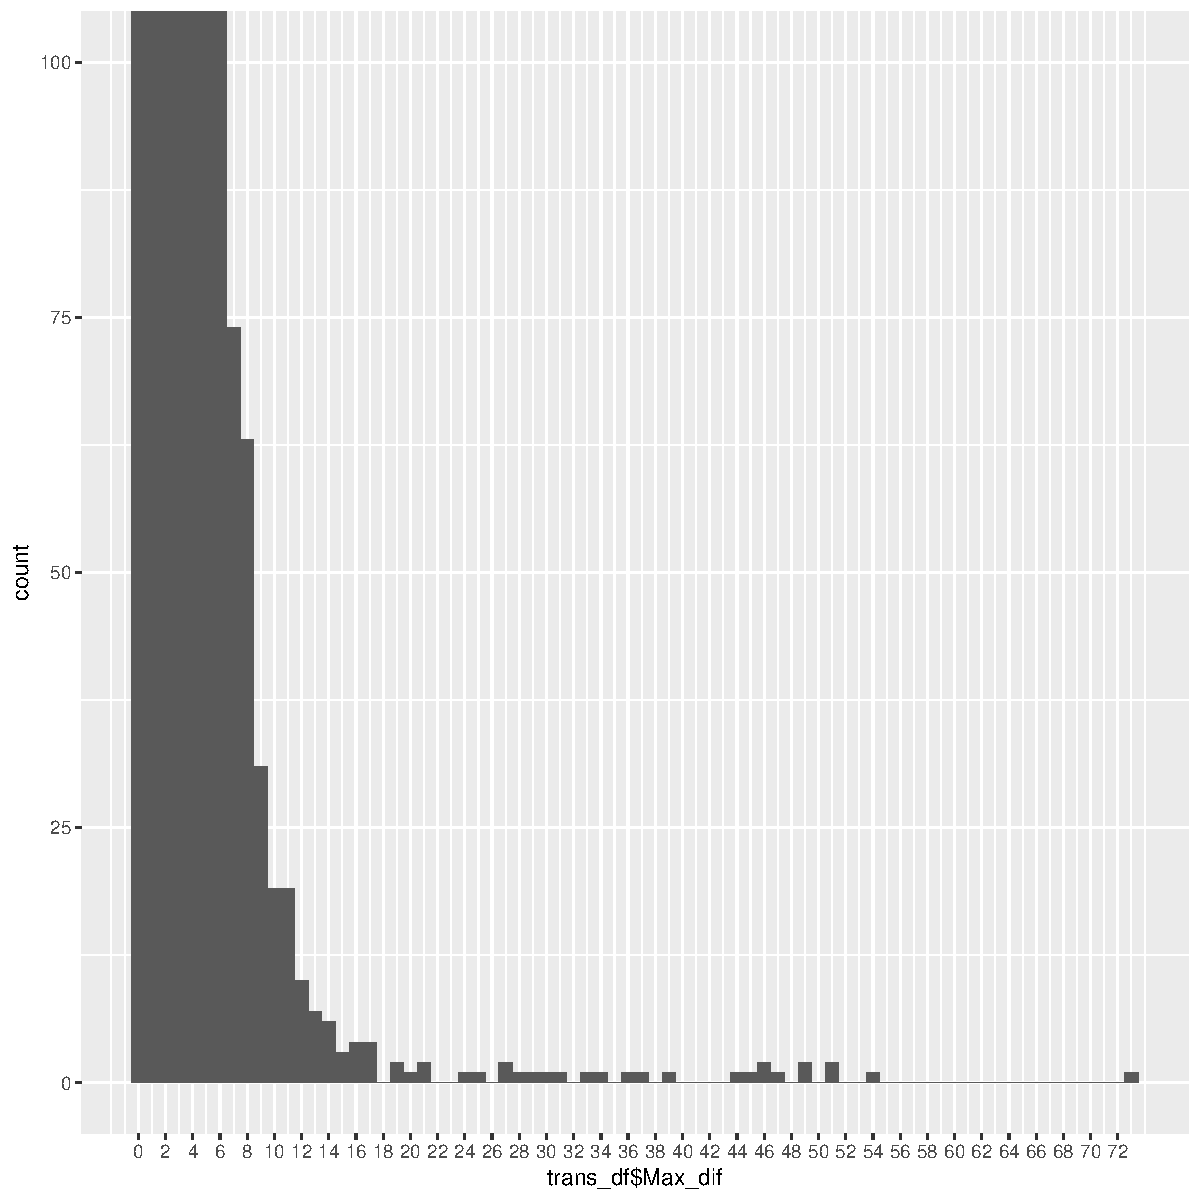
\includegraphics[width=.4\linewidth]{figure/minimal-plots-1} 
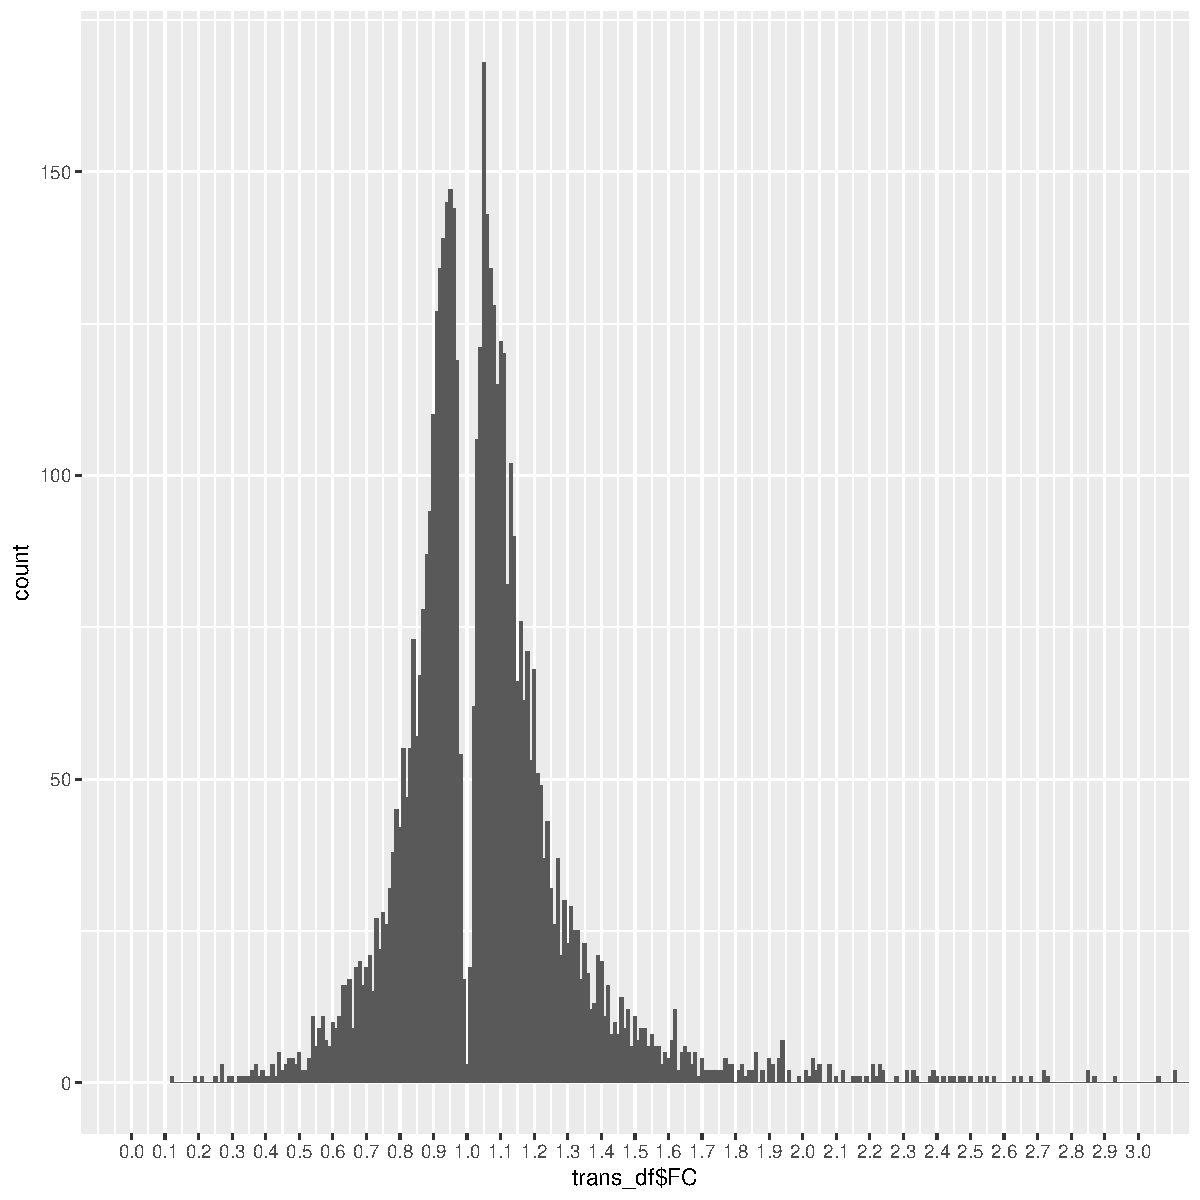
\includegraphics[width=.4\linewidth]{figure/minimal-plots-2} 

}



\end{knitrout}

\section{Llistes}
I comencem les comparacions:

\begin{knitrout}
\definecolor{shadecolor}{rgb}{0.969, 0.969, 0.969}\color{fgcolor}\begin{kframe}
\begin{alltt}
\hlstd{trans_df_FC} \hlkwb{<-} \hlstd{trans_df[}\hlopt{!}\hlkwd{is.na}\hlstd{(trans_df}\hlopt{$}\hlstd{FC),]}

\hlstd{df_10G_tss} \hlkwb{<-} \hlstd{df_10G[df_10G}\hlopt{$}\hlstd{X5.cov} \hlopt{>} \hlnum{10}\hlstd{,]}
\hlstd{df_10G_ORF} \hlkwb{<-} \hlstd{df_10G[df_10G}\hlopt{$}\hlstd{Gene.cov} \hlopt{>} \hlnum{10}\hlstd{,]}
\hlstd{df_10G_tts} \hlkwb{<-} \hlstd{df_10G[df_10G}\hlopt{$}\hlstd{X3.cov} \hlopt{>} \hlnum{10}\hlstd{,]}
\hlstd{df_10G_filtered} \hlkwb{<-} \hlstd{df_10G[df_10G}\hlopt{$}\hlstd{X5.cov} \hlopt{>} \hlnum{10} \hlopt{|} \hlstd{df_10G}\hlopt{$}\hlstd{Gene.cov} \hlopt{>} \hlnum{10}\hlstd{,]}

\hlkwd{table}\hlstd{(df_10G_tts[}\hlopt{!}\hlkwd{is.na}\hlstd{(df_10G_tts}\hlopt{$}\hlstd{FC),]}\hlopt{$}\hlstd{Gene} \hlopt \hlstd{trans_df_FC}\hlopt{$}\hlstd{ID[trans_df_FC}\hlopt{$}\hlstd{FC} \hlopt{>} \hlnum{1}\hlstd{])}
\end{alltt}
\begin{verbatim}
## < table of extent 0 >
\end{verbatim}
\begin{alltt}
\hlstd{df_10G_tts[df_10G_tts}\hlopt{$}\hlstd{Gene} \hlopt \hlstd{trans_df_FC}\hlopt{$}\hlstd{ID[trans_df_FC}\hlopt{$}\hlstd{FC} \hlopt{>} \hlnum{1}\hlstd{],}\hlstr{"Annotations"}\hlstd{]}
\end{alltt}
\begin{verbatim}
##  [1] ID=PF3D7_0100300;description=erythrocyte membrane protein 1%2C PfEMP1                
##  [2] ID=PF3D7_0220800;description=cytoadherence linked asexual protein 2                  
##  [3] ID=PF3D7_0402000;description=Plasmodium exported protein (PHISTa)%2C unknown function
##  [4] ID=PF3D7_0402000;description=Plasmodium exported protein (PHISTa)%2C unknown function
##  [5] ID=PF3D7_0421600;description=erythrocyte membrane protein 1 (PfEMP1)-like pseudogene 
##  [6] ID=PF3D7_0421700;description=conserved Plasmodium protein%2C unknown function        
##  [7] ID=PF3D7_0421700;description=conserved Plasmodium protein%2C unknown function        
##  [8] ID=PF3D7_0532600;description=Plasmodium exported protein%2C unknown function         
##  [9] ID=PF3D7_0532600;description=Plasmodium exported protein%2C unknown function         
## [10] ID=PF3D7_0711700;description=erythrocyte membrane protein 1%2C PfEMP1                
## [11] ID=PF3D7_0711900;description=rifin%2C pseudogene                                     
## [12] ID=PF3D7_0732900;description=rifin                                                   
## [13] ID=PF3D7_0800800;description=Plasmodium exported protein (hyp7)%2C unknown function  
## [14] ID=PF3D7_1040500;description=rifin                                                   
## [15] ID=PF3D7_1040700;description=rifin                                                   
## [16] ID=PF3D7_1300400;description=rifin                                                   
## [17] ID=PF3D7_1300500;description=rifin                                                   
## [18] ID=PF3D7_1300600;description=rifin                                                   
## [19] ID=PF3D7_1301400;description=Plasmodium exported protein (hyp12)%2C unknown function 
## [20] ID=PF3D7_1301500;description=Plasmodium exported protein (PHISTa)%2C unknown function
## [21] ID=PF3D7_1371900;description=Plasmodium exported protein%2C unknown function         
## 51 Levels: ID=PF3D7_0100200;description=rifin ...
\end{verbatim}
\begin{alltt}
\hlstd{df_10G_tts[df_10G_tts}\hlopt{$}\hlstd{Gene} \hlopt \hlstd{trans_df_FC}\hlopt{$}\hlstd{ID[trans_df_FC}\hlopt{$}\hlstd{FC} \hlopt{<} \hlnum{1}\hlstd{],}\hlstr{"Annotations"}\hlstd{]}
\end{alltt}
\begin{verbatim}
## [1] ID=PF3D7_0712000;description=erythrocyte membrane protein 1%2C PfEMP1
## [2] ID=PF3D7_0937800;description=erythrocyte membrane protein 1%2C PfEMP1
## [3] ID=PF3D7_1040600;description=rifin                                   
## [4] ID=PF3D7_1040600;description=rifin                                   
## [5] ID=PF3D7_1301600;description=erythrocyte binding antigen-140         
## 51 Levels: ID=PF3D7_0100200;description=rifin ...
\end{verbatim}
\begin{alltt}
\hlkwd{table}\hlstd{(df_10G_tss[}\hlopt{!}\hlkwd{is.na}\hlstd{(df_10G_tss}\hlopt{$}\hlstd{FC),]}\hlopt{$}\hlstd{Gene} \hlopt \hlstd{trans_df_FC}\hlopt{$}\hlstd{ID[trans_df_FC}\hlopt{$}\hlstd{FC} \hlopt{>} \hlnum{1}\hlstd{])}
\end{alltt}
\begin{verbatim}
## < table of extent 0 >
\end{verbatim}
\begin{alltt}
\hlstd{df_10G_tss[df_10G_tss}\hlopt{$}\hlstd{Gene} \hlopt \hlstd{trans_df_FC}\hlopt{$}\hlstd{ID[trans_df_FC}\hlopt{$}\hlstd{FC} \hlopt{>} \hlnum{1}\hlstd{],}\hlstr{"Annotations"}\hlstd{]}
\end{alltt}
\begin{verbatim}
##  [1] ID=PF3D7_0220800;description=cytoadherence linked asexual protein 2                                     
##  [2] ID=PF3D7_0302500;description=cytoadherence linked asexual protein 3.1                                   
##  [3] ID=PF3D7_0324800;description=rifin                                                                      
##  [4] ID=PF3D7_0532600;description=Plasmodium exported protein%2C unknown function                            
##  [5] ID=PF3D7_0711700;description=erythrocyte membrane protein 1%2C PfEMP1                                   
##  [6] ID=PF3D7_0711900;description=rifin%2C pseudogene                                                        
##  [7] ID=PF3D7_0800800;description=Plasmodium exported protein (hyp7)%2C unknown function                     
##  [8] ID=PF3D7_0800800;description=Plasmodium exported protein (hyp7)%2C unknown function                     
##  [9] ID=PF3D7_1040500;description=rifin                                                                      
## [10] ID=PF3D7_1040700;description=rifin                                                                      
## [11] ID=PF3D7_1300500;description=rifin                                                                      
## [12] ID=PF3D7_1301300;description=Plasmodium exported protein (PHISTa-like)%2C unknown function%2C pseudogene
## [13] ID=PF3D7_1301500;description=Plasmodium exported protein (PHISTa)%2C unknown function                   
## [14] ID=PF3D7_1301500;description=Plasmodium exported protein (PHISTa)%2C unknown function                   
## [15] ID=PF3D7_1372000;description=Plasmodium exported protein (PHISTa)%2C unknown function                   
## 51 Levels: ID=PF3D7_0100200;description=rifin ...
\end{verbatim}
\begin{alltt}
\hlstd{df_10G_tss[df_10G_tss}\hlopt{$}\hlstd{Gene} \hlopt \hlstd{trans_df_FC}\hlopt{$}\hlstd{ID[trans_df_FC}\hlopt{$}\hlstd{FC} \hlopt{<} \hlnum{1}\hlstd{],}\hlstr{"Annotations"}\hlstd{]}
\end{alltt}
\begin{verbatim}
## [1] ID=PF3D7_1040600;description=rifin
## 51 Levels: ID=PF3D7_0100200;description=rifin ...
\end{verbatim}
\begin{alltt}
\hlkwd{table}\hlstd{(df_10G_ORF[}\hlopt{!}\hlkwd{is.na}\hlstd{(df_10G_ORF}\hlopt{$}\hlstd{FC),]}\hlopt{$}\hlstd{Gene} \hlopt \hlstd{trans_df_FC}\hlopt{$}\hlstd{ID[trans_df_FC}\hlopt{$}\hlstd{FC} \hlopt{>} \hlnum{1}\hlstd{])}
\end{alltt}
\begin{verbatim}
## < table of extent 0 >
\end{verbatim}
\begin{alltt}
\hlstd{df_10G_ORF[df_10G_ORF}\hlopt{$}\hlstd{Gene} \hlopt \hlstd{trans_df_FC}\hlopt{$}\hlstd{ID[trans_df_FC}\hlopt{$}\hlstd{FC} \hlopt{>} \hlnum{1}\hlstd{],}\hlstr{"Annotations"}\hlstd{]}
\end{alltt}
\begin{verbatim}
##  [1] ID=PF3D7_0100200;description=rifin                                                                      
##  [2] ID=PF3D7_0100300;description=erythrocyte membrane protein 1%2C PfEMP1                                   
##  [3] ID=PF3D7_0100400;description=rifin                                                                      
##  [4] ID=PF3D7_0220800;description=cytoadherence linked asexual protein 2                                     
##  [5] ID=PF3D7_0302500;description=cytoadherence linked asexual protein 3.1                                   
##  [6] ID=PF3D7_0302500;description=cytoadherence linked asexual protein 3.1                                   
##  [7] ID=PF3D7_0324800;description=rifin                                                                      
##  [8] ID=PF3D7_0402000;description=Plasmodium exported protein (PHISTa)%2C unknown function                   
##  [9] ID=PF3D7_0421600;description=erythrocyte membrane protein 1 (PfEMP1)-like pseudogene                    
## [10] ID=PF3D7_0421700;description=conserved Plasmodium protein%2C unknown function                           
## [11] ID=PF3D7_0711700;description=erythrocyte membrane protein 1%2C PfEMP1                                   
## [12] ID=PF3D7_0711700;description=erythrocyte membrane protein 1%2C PfEMP1                                   
## [13] ID=PF3D7_0732900;description=rifin                                                                      
## [14] ID=PF3D7_0800800;description=Plasmodium exported protein (hyp7)%2C unknown function                     
## [15] ID=PF3D7_0808900;description=rifin                                                                      
## [16] ID=PF3D7_1040500;description=rifin                                                                      
## [17] ID=PF3D7_1040700;description=rifin                                                                      
## [18] ID=PF3D7_1240600;description=erythrocyte membrane protein 1%2C PfEMP1                                   
## [19] ID=PF3D7_1240600;description=erythrocyte membrane protein 1%2C PfEMP1                                   
## [20] ID=PF3D7_1300200;description=rifin                                                                      
## [21] ID=PF3D7_1300400;description=rifin                                                                      
## [22] ID=PF3D7_1300500;description=rifin                                                                      
## [23] ID=PF3D7_1300600;description=rifin                                                                      
## [24] ID=PF3D7_1301300;description=Plasmodium exported protein (PHISTa-like)%2C unknown function%2C pseudogene
## [25] ID=PF3D7_1301500;description=Plasmodium exported protein (PHISTa)%2C unknown function                   
## [26] ID=PF3D7_1371900;description=Plasmodium exported protein%2C unknown function                            
## [27] ID=PF3D7_1372000;description=Plasmodium exported protein (PHISTa)%2C unknown function                   
## 51 Levels: ID=PF3D7_0100200;description=rifin ...
\end{verbatim}
\begin{alltt}
\hlstd{df_10G_ORF[df_10G_ORF}\hlopt{$}\hlstd{Gene} \hlopt \hlstd{trans_df_FC}\hlopt{$}\hlstd{ID[trans_df_FC}\hlopt{$}\hlstd{FC} \hlopt{<} \hlnum{1}\hlstd{],}\hlstr{"Annotations"}\hlstd{]}
\end{alltt}
\begin{verbatim}
##  [1] ID=PF3D7_0712000;description=erythrocyte membrane protein 1%2C PfEMP1
##  [2] ID=PF3D7_0712000;description=erythrocyte membrane protein 1%2C PfEMP1
##  [3] ID=PF3D7_0733000;description=erythrocyte membrane protein 1%2C PfEMP1
##  [4] ID=PF3D7_0733000;description=erythrocyte membrane protein 1%2C PfEMP1
##  [5] ID=PF3D7_0808800;description=rifin                                   
##  [6] ID=PF3D7_0937800;description=erythrocyte membrane protein 1%2C PfEMP1
##  [7] ID=PF3D7_0937800;description=erythrocyte membrane protein 1%2C PfEMP1
##  [8] ID=PF3D7_1040600;description=rifin                                   
##  [9] ID=PF3D7_1041300;description=erythrocyte membrane protein 1%2C PfEMP1
## [10] ID=PF3D7_1041300;description=erythrocyte membrane protein 1%2C PfEMP1
## [11] ID=PF3D7_1300300;description=erythrocyte membrane protein 1%2C PfEMP1
## [12] ID=PF3D7_1301600;description=erythrocyte binding antigen-140         
## [13] ID=PF3D7_1373500;description=erythrocyte membrane protein 1%2C PfEMP1
## 51 Levels: ID=PF3D7_0100200;description=rifin ...
\end{verbatim}
\begin{alltt}
\hlkwd{table}\hlstd{(df_10G_filtered[}\hlopt{!}\hlkwd{is.na}\hlstd{(df_10G_filtered}\hlopt{$}\hlstd{FC),]}\hlopt{$}\hlstd{Gene} \hlopt \hlstd{trans_df_FC}\hlopt{$}\hlstd{ID[trans_df_FC}\hlopt{$}\hlstd{FC} \hlopt{>} \hlnum{1}\hlstd{])}
\end{alltt}
\begin{verbatim}
## < table of extent 0 >
\end{verbatim}
\begin{alltt}
\hlstd{df_10G_filtered[df_10G_filtered}\hlopt{$}\hlstd{Gene} \hlopt \hlstd{trans_df_FC}\hlopt{$}\hlstd{ID[trans_df_FC}\hlopt{$}\hlstd{FC} \hlopt{>} \hlnum{1}\hlstd{],}\hlstr{"Annotations"}\hlstd{]}
\end{alltt}
\begin{verbatim}
##  [1] ID=PF3D7_0100200;description=rifin                                                                      
##  [2] ID=PF3D7_0100300;description=erythrocyte membrane protein 1%2C PfEMP1                                   
##  [3] ID=PF3D7_0100400;description=rifin                                                                      
##  [4] ID=PF3D7_0220800;description=cytoadherence linked asexual protein 2                                     
##  [5] ID=PF3D7_0302500;description=cytoadherence linked asexual protein 3.1                                   
##  [6] ID=PF3D7_0302500;description=cytoadherence linked asexual protein 3.1                                   
##  [7] ID=PF3D7_0324800;description=rifin                                                                      
##  [8] ID=PF3D7_0402000;description=Plasmodium exported protein (PHISTa)%2C unknown function                   
##  [9] ID=PF3D7_0421600;description=erythrocyte membrane protein 1 (PfEMP1)-like pseudogene                    
## [10] ID=PF3D7_0421700;description=conserved Plasmodium protein%2C unknown function                           
## [11] ID=PF3D7_0532600;description=Plasmodium exported protein%2C unknown function                            
## [12] ID=PF3D7_0711700;description=erythrocyte membrane protein 1%2C PfEMP1                                   
## [13] ID=PF3D7_0711700;description=erythrocyte membrane protein 1%2C PfEMP1                                   
## [14] ID=PF3D7_0711900;description=rifin%2C pseudogene                                                        
## [15] ID=PF3D7_0732900;description=rifin                                                                      
## [16] ID=PF3D7_0800800;description=Plasmodium exported protein (hyp7)%2C unknown function                     
## [17] ID=PF3D7_0800800;description=Plasmodium exported protein (hyp7)%2C unknown function                     
## [18] ID=PF3D7_0800800;description=Plasmodium exported protein (hyp7)%2C unknown function                     
## [19] ID=PF3D7_0808900;description=rifin                                                                      
## [20] ID=PF3D7_1040500;description=rifin                                                                      
## [21] ID=PF3D7_1040500;description=rifin                                                                      
## [22] ID=PF3D7_1040700;description=rifin                                                                      
## [23] ID=PF3D7_1240600;description=erythrocyte membrane protein 1%2C PfEMP1                                   
## [24] ID=PF3D7_1240600;description=erythrocyte membrane protein 1%2C PfEMP1                                   
## [25] ID=PF3D7_1300200;description=rifin                                                                      
## [26] ID=PF3D7_1300400;description=rifin                                                                      
## [27] ID=PF3D7_1300500;description=rifin                                                                      
## [28] ID=PF3D7_1300500;description=rifin                                                                      
## [29] ID=PF3D7_1300600;description=rifin                                                                      
## [30] ID=PF3D7_1301300;description=Plasmodium exported protein (PHISTa-like)%2C unknown function%2C pseudogene
## [31] ID=PF3D7_1301500;description=Plasmodium exported protein (PHISTa)%2C unknown function                   
## [32] ID=PF3D7_1301500;description=Plasmodium exported protein (PHISTa)%2C unknown function                   
## [33] ID=PF3D7_1371900;description=Plasmodium exported protein%2C unknown function                            
## [34] ID=PF3D7_1372000;description=Plasmodium exported protein (PHISTa)%2C unknown function                   
## [35] ID=PF3D7_1372000;description=Plasmodium exported protein (PHISTa)%2C unknown function                   
## 51 Levels: ID=PF3D7_0100200;description=rifin ...
\end{verbatim}
\begin{alltt}
\hlstd{df_10G_filtered[df_10G_filtered}\hlopt{$}\hlstd{Gene} \hlopt \hlstd{trans_df_FC}\hlopt{$}\hlstd{ID[trans_df_FC}\hlopt{$}\hlstd{FC} \hlopt{<} \hlnum{1}\hlstd{],}\hlstr{"Annotations"}\hlstd{]}
\end{alltt}
\begin{verbatim}
##  [1] ID=PF3D7_0712000;description=erythrocyte membrane protein 1%2C PfEMP1
##  [2] ID=PF3D7_0712000;description=erythrocyte membrane protein 1%2C PfEMP1
##  [3] ID=PF3D7_0733000;description=erythrocyte membrane protein 1%2C PfEMP1
##  [4] ID=PF3D7_0733000;description=erythrocyte membrane protein 1%2C PfEMP1
##  [5] ID=PF3D7_0808800;description=rifin                                   
##  [6] ID=PF3D7_0937800;description=erythrocyte membrane protein 1%2C PfEMP1
##  [7] ID=PF3D7_0937800;description=erythrocyte membrane protein 1%2C PfEMP1
##  [8] ID=PF3D7_1040600;description=rifin                                   
##  [9] ID=PF3D7_1040600;description=rifin                                   
## [10] ID=PF3D7_1041300;description=erythrocyte membrane protein 1%2C PfEMP1
## [11] ID=PF3D7_1041300;description=erythrocyte membrane protein 1%2C PfEMP1
## [12] ID=PF3D7_1300300;description=erythrocyte membrane protein 1%2C PfEMP1
## [13] ID=PF3D7_1301600;description=erythrocyte binding antigen-140         
## [14] ID=PF3D7_1373500;description=erythrocyte membrane protein 1%2C PfEMP1
## 51 Levels: ID=PF3D7_0100200;description=rifin ...
\end{verbatim}
\begin{alltt}
\hlstd{df_1.2B_tss} \hlkwb{<-} \hlstd{df_1.2B[df_1.2B}\hlopt{$}\hlstd{X5.cov} \hlopt{>} \hlnum{10}\hlstd{,]}
\hlstd{df_1.2B_ORF} \hlkwb{<-} \hlstd{df_1.2B[df_1.2B}\hlopt{$}\hlstd{Gene.cov} \hlopt{>} \hlnum{10}\hlstd{,]}
\hlstd{df_1.2B_tts} \hlkwb{<-} \hlstd{df_1.2B[df_1.2B}\hlopt{$}\hlstd{X3.cov}\hlopt{>} \hlnum{10}\hlstd{,]}
\hlstd{df_1.2B_filtered} \hlkwb{<-} \hlstd{df_1.2B[df_1.2B}\hlopt{$}\hlstd{X5.cov} \hlopt{>} \hlnum{10} \hlopt{|} \hlstd{df_1.2B}\hlopt{$}\hlstd{Gene.cov} \hlopt{>} \hlnum{10}\hlstd{,]}

\hlkwd{table}\hlstd{(df_1.2B_tss[}\hlopt{!}\hlkwd{is.na}\hlstd{(df_1.2B_tss}\hlopt{$}\hlstd{FC),]}\hlopt{$}\hlstd{Gene} \hlopt \hlstd{trans_df_FC}\hlopt{$}\hlstd{ID[trans_df_FC}\hlopt{$}\hlstd{FC} \hlopt{<} \hlnum{1}\hlstd{])}
\end{alltt}
\begin{verbatim}
## < table of extent 0 >
\end{verbatim}
\begin{alltt}
\hlstd{df_1.2B_tss[df_1.2B_tss}\hlopt{$}\hlstd{Gene} \hlopt \hlstd{trans_df_FC}\hlopt{$}\hlstd{ID[trans_df_FC}\hlopt{$}\hlstd{FC} \hlopt{<} \hlnum{1}\hlstd{],}\hlstr{"Annotations"}\hlstd{]}
\end{alltt}
\begin{verbatim}
##  [1] ID=PF3D7_0302200;description=cytoadherence linked asexual protein 3.2              
##  [2] ID=PF3D7_0421100;description=erythrocyte membrane protein 1%2C PfEMP1              
##  [3] ID=PF3D7_0421100;description=erythrocyte membrane protein 1%2C PfEMP1              
##  [4] ID=PF3D7_0425900;description=rifin                                                 
##  [5] ID=PF3D7_1100500;description=rifin                                                 
##  [6] ID=PF3D7_1139100;description=RNA-binding protein%2C putative                       
##  [7] ID=PF3D7_1301600;description=erythrocyte binding antigen-140                       
##  [8] ID=PF3D7_1301600;description=erythrocyte binding antigen-140                       
##  [9] ID=PF3D7_1301700;description=Plasmodium exported protein (hyp8)%2C unknown function
## [10] ID=PF3D7_1301700;description=Plasmodium exported protein (hyp8)%2C unknown function
## 42 Levels: ID=PF3D7_0115000;description=surface-associated interspersed protein 1.3 (SURFIN 1.3) ...
\end{verbatim}
\begin{alltt}
\hlstd{df_1.2B_tss[df_1.2B_tss}\hlopt{$}\hlstd{Gene} \hlopt \hlstd{trans_df_FC}\hlopt{$}\hlstd{ID[trans_df_FC}\hlopt{$}\hlstd{FC} \hlopt{>} \hlnum{1}\hlstd{],}\hlstr{"Annotations"}\hlstd{]}
\end{alltt}
\begin{verbatim}
## [1] ID=PF3D7_0223400;description=rifin                                   
## [2] ID=PF3D7_0421200;description=rifin                                   
## [3] ID=PF3D7_1100100;description=erythrocyte membrane protein 1%2C PfEMP1
## [4] ID=PF3D7_1100100;description=erythrocyte membrane protein 1%2C PfEMP1
## 42 Levels: ID=PF3D7_0115000;description=surface-associated interspersed protein 1.3 (SURFIN 1.3) ...
\end{verbatim}
\begin{alltt}
\hlkwd{table}\hlstd{(df_1.2B_tts[}\hlopt{!}\hlkwd{is.na}\hlstd{(df_1.2B_tts}\hlopt{$}\hlstd{FC),]}\hlopt{$}\hlstd{Gene} \hlopt \hlstd{trans_df_FC}\hlopt{$}\hlstd{ID[trans_df_FC}\hlopt{$}\hlstd{FC} \hlopt{<} \hlnum{1}\hlstd{])}
\end{alltt}
\begin{verbatim}
## < table of extent 0 >
\end{verbatim}
\begin{alltt}
\hlstd{df_1.2B_tts[df_1.2B_tts}\hlopt{$}\hlstd{Gene} \hlopt \hlstd{trans_df_FC}\hlopt{$}\hlstd{ID[trans_df_FC}\hlopt{$}\hlstd{FC} \hlopt{<} \hlnum{1}\hlstd{],}\hlstr{"Annotations"}\hlstd{]}
\end{alltt}
\begin{verbatim}
##  [1] ID=PF3D7_0223500;description=erythrocyte membrane protein 1%2C PfEMP1              
##  [2] ID=PF3D7_0302100;description=serine/threonine protein kinase                       
##  [3] ID=PF3D7_0302200;description=cytoadherence linked asexual protein 3.2              
##  [4] ID=PF3D7_0302200;description=cytoadherence linked asexual protein 3.2              
##  [5] ID=PF3D7_0421300;description=erythrocyte membrane protein 1%2C PfEMP1              
##  [6] ID=PF3D7_0731800;description=alpha/beta hydrolase%2C putative                      
##  [7] ID=PF3D7_0731800;description=alpha/beta hydrolase%2C putative                      
##  [8] ID=PF3D7_1100300;description=rifin                                                 
##  [9] ID=PF3D7_1100300;description=rifin                                                 
## [10] ID=PF3D7_1240000;description=3-hydroxyisobutyryl-coenzyme A hydrolase%2C putative  
## [11] ID=PF3D7_1240100;description=early transcribed membrane protein 12                 
## [12] ID=PF3D7_1301700;description=Plasmodium exported protein (hyp8)%2C unknown function
## 42 Levels: ID=PF3D7_0115000;description=surface-associated interspersed protein 1.3 (SURFIN 1.3) ...
\end{verbatim}
\begin{alltt}
\hlstd{df_1.2B_tts[df_1.2B_tts}\hlopt{$}\hlstd{Gene} \hlopt \hlstd{trans_df_FC}\hlopt{$}\hlstd{ID[trans_df_FC}\hlopt{$}\hlstd{FC} \hlopt{>} \hlnum{1}\hlstd{],}\hlstr{"Annotations"}\hlstd{]}
\end{alltt}
\begin{verbatim}
## [1] ID=PF3D7_0115600;description=rifin                                         
## [2] ID=PF3D7_0223400;description=rifin                                         
## [3] ID=PF3D7_0421200;description=rifin                                         
## [4] ID=PF3D7_0421200;description=rifin                                         
## [5] ID=PF3D7_1039000;description=serine/threonine protein kinase%2C FIKK family
## 42 Levels: ID=PF3D7_0115000;description=surface-associated interspersed protein 1.3 (SURFIN 1.3) ...
\end{verbatim}
\begin{alltt}
\hlkwd{table}\hlstd{(df_1.2B_ORF[}\hlopt{!}\hlkwd{is.na}\hlstd{(df_1.2B_ORF}\hlopt{$}\hlstd{FC),]}\hlopt{$}\hlstd{Gene} \hlopt \hlstd{trans_df_FC}\hlopt{$}\hlstd{ID[trans_df_FC}\hlopt{$}\hlstd{FC} \hlopt{<} \hlnum{1}\hlstd{])}
\end{alltt}
\begin{verbatim}
## < table of extent 0 >
\end{verbatim}
\begin{alltt}
\hlstd{df_1.2B_ORF[df_1.2B_ORF}\hlopt{$}\hlstd{Gene} \hlopt \hlstd{trans_df_FC}\hlopt{$}\hlstd{ID[trans_df_FC}\hlopt{$}\hlstd{FC} \hlopt{<} \hlnum{1}\hlstd{],}\hlstr{"Annotations"}\hlstd{]}
\end{alltt}
\begin{verbatim}
##  [1] ID=PF3D7_0115700;description=erythrocyte membrane protein 1%2C PfEMP1              
##  [2] ID=PF3D7_0302100;description=serine/threonine protein kinase                       
##  [3] ID=PF3D7_0302200;description=cytoadherence linked asexual protein 3.2              
##  [4] ID=PF3D7_0302200;description=cytoadherence linked asexual protein 3.2              
##  [5] ID=PF3D7_0421100;description=erythrocyte membrane protein 1%2C PfEMP1              
##  [6] ID=PF3D7_0421300;description=erythrocyte membrane protein 1%2C PfEMP1              
##  [7] ID=PF3D7_0421300;description=erythrocyte membrane protein 1%2C PfEMP1              
##  [8] ID=PF3D7_0425900;description=rifin                                                 
##  [9] ID=PF3D7_0731800;description=alpha/beta hydrolase%2C putative                      
## [10] ID=PF3D7_1100300;description=rifin                                                 
## [11] ID=PF3D7_1100500;description=rifin                                                 
## [12] ID=PF3D7_1139100;description=RNA-binding protein%2C putative                       
## [13] ID=PF3D7_1255200;description=erythrocyte membrane protein 1%2C PfEMP1              
## [14] ID=PF3D7_1301600;description=erythrocyte binding antigen-140                       
## [15] ID=PF3D7_1301700;description=Plasmodium exported protein (hyp8)%2C unknown function
## 42 Levels: ID=PF3D7_0115000;description=surface-associated interspersed protein 1.3 (SURFIN 1.3) ...
\end{verbatim}
\begin{alltt}
\hlstd{df_1.2B_ORF[df_1.2B_ORF}\hlopt{$}\hlstd{Gene} \hlopt \hlstd{trans_df_FC}\hlopt{$}\hlstd{ID[trans_df_FC}\hlopt{$}\hlstd{FC} \hlopt{>} \hlnum{1}\hlstd{],}\hlstr{"Annotations"}\hlstd{]}
\end{alltt}
\begin{verbatim}
## [1] ID=PF3D7_0115600;description=rifin                                         
## [2] ID=PF3D7_0421200;description=rifin                                         
## [3] ID=PF3D7_1039000;description=serine/threonine protein kinase%2C FIKK family
## [4] ID=PF3D7_1100100;description=erythrocyte membrane protein 1%2C PfEMP1      
## 42 Levels: ID=PF3D7_0115000;description=surface-associated interspersed protein 1.3 (SURFIN 1.3) ...
\end{verbatim}
\begin{alltt}
\hlkwd{table}\hlstd{(df_1.2B_filtered[}\hlopt{!}\hlkwd{is.na}\hlstd{(df_1.2B_filtered}\hlopt{$}\hlstd{FC),]}\hlopt{$}\hlstd{Gene} \hlopt \hlstd{trans_df_FC}\hlopt{$}\hlstd{ID[trans_df_FC}\hlopt{$}\hlstd{FC} \hlopt{<} \hlnum{1}\hlstd{])}
\end{alltt}
\begin{verbatim}
## < table of extent 0 >
\end{verbatim}
\begin{alltt}
\hlstd{df_1.2B_ORF[df_1.2B_filtered}\hlopt{$}\hlstd{Gene} \hlopt \hlstd{trans_df_FC}\hlopt{$}\hlstd{ID[trans_df_FC}\hlopt{$}\hlstd{FC} \hlopt{<} \hlnum{1}\hlstd{],}\hlstr{"Annotations"}\hlstd{]}
\end{alltt}
\begin{verbatim}
##  [1] ID=PF3D7_0302100;description=serine/threonine protein kinase         
##  [2] ID=PF3D7_0421100;description=erythrocyte membrane protein 1%2C PfEMP1
##  [3] ID=PF3D7_0421200;description=rifin                                   
##  [4] ID=PF3D7_0421300;description=erythrocyte membrane protein 1%2C PfEMP1
##  [5] ID=PF3D7_0425800;description=erythrocyte membrane protein 1%2C PfEMP1
##  [6] ID=PF3D7_0425800;description=erythrocyte membrane protein 1%2C PfEMP1
##  [7] ID=PF3D7_0731800;description=alpha/beta hydrolase%2C putative        
##  [8] ID=PF3D7_0731900;description=rifin%2C pseudogene                     
##  [9] ID=PF3D7_1100300;description=rifin                                   
## [10] ID=PF3D7_1100400;description=rifin                                   
## [11] ID=PF3D7_1139100;description=RNA-binding protein%2C putative         
## [12] <NA>                                                                 
## [13] <NA>                                                                 
## [14] <NA>                                                                 
## [15] <NA>                                                                 
## [16] <NA>                                                                 
## [17] <NA>                                                                 
## [18] <NA>                                                                 
## [19] <NA>                                                                 
## [20] <NA>                                                                 
## 42 Levels: ID=PF3D7_0115000;description=surface-associated interspersed protein 1.3 (SURFIN 1.3) ...
\end{verbatim}
\begin{alltt}
\hlstd{df_1.2B_ORF[df_1.2B_filtered}\hlopt{$}\hlstd{Gene} \hlopt \hlstd{trans_df_FC}\hlopt{$}\hlstd{ID[trans_df_FC}\hlopt{$}\hlstd{FC} \hlopt{>} \hlnum{1}\hlstd{],}\hlstr{"Annotations"}\hlstd{]}
\end{alltt}
\begin{verbatim}
## [1] ID=PF3D7_0115700;description=erythrocyte membrane protein 1%2C PfEMP1              
## [2] ID=PF3D7_0401500;description=stevor%2C pseudogene                                  
## [3] ID=PF3D7_0425900;description=rifin                                                 
## [4] ID=PF3D7_0500300;description=rifin%2C pseudogene                                   
## [5] ID=PF3D7_1255100;description=rifin                                                 
## [6] ID=PF3D7_1301600;description=erythrocyte binding antigen-140                       
## [7] ID=PF3D7_1301700;description=Plasmodium exported protein (hyp8)%2C unknown function
## 42 Levels: ID=PF3D7_0115000;description=surface-associated interspersed protein 1.3 (SURFIN 1.3) ...
\end{verbatim}
\end{kframe}
\end{knitrout}



\begin{knitrout}
\definecolor{shadecolor}{rgb}{0.969, 0.969, 0.969}\color{fgcolor}\begin{kframe}
\begin{alltt}
\hlkwd{length}\hlstd{(trans_df}\hlopt{$}\hlstd{ID[trans_df}\hlopt{$}\hlstd{FC} \hlopt{>} \hlnum{1}\hlstd{])}
\end{alltt}
\begin{verbatim}
## [1] 2947
\end{verbatim}
\begin{alltt}
\hlkwd{length}\hlstd{(trans_df}\hlopt{$}\hlstd{ID[trans_df}\hlopt{$}\hlstd{FC} \hlopt{<} \hlnum{1}\hlstd{])}
\end{alltt}
\begin{verbatim}
## [1] 2449
\end{verbatim}
\begin{alltt}
\hlkwd{length}\hlstd{(trans_df}\hlopt{$}\hlstd{ID)}
\end{alltt}
\begin{verbatim}
## [1] 5267
\end{verbatim}
\begin{alltt}
\hlnum{2449}\hlopt{+}\hlnum{2947}
\end{alltt}
\begin{verbatim}
## [1] 5396
\end{verbatim}
\end{kframe}
\end{knitrout}



\end{document}
